% TEMPLATE for Usenix papers, specifically to meet requirements of
%  USENIX '05
% originally a template for producing IEEE-format articles using LaTeX.
%   written by Matthew Ward, CS Department, Worcester Polytechnic Institute.
% adapted by David Beazley for his excellent SWIG paper in Proceedings,
%   Tcl 96
% turned into a smartass generic template by De Clarke, with thanks to
%   both the above pioneers
% use at your own risk.  Complaints to /dev/null.
% make it two column with no page numbering, default is 10 point

% Munged by Fred Douglis <douglis@research.att.com> 10/97 to separate
% the .sty file from the LaTeX source template, so that people can
% more easily include the .sty file into an existing document.  Also
% changed to more closely follow the style guidelines as represented
% by the Word sample file. 
% This version uses the latex2e styles, not the very ancient 2.09 stuff.
\documentclass[letterpaper,twocolumn,10pt]{article}
\usepackage{usenix,epsfig,endnotes,url}
\begin{document}

%don't want date printed
\date{}

%make title bold and 14 pt font (Latex default is non-bold, 16 pt)
\title{  Chukwa: A large-scale monitoring system}

%for single author (just remove % characters)
\author{
{\rm Jerome Boulon}\\
{\rm jboulon@yahoo-inc.com}\\
Yahoo!, inc
\and
{\rm Andy Konwinski}\\
{\rm andyk@cs.berkeley.edu}\\
UC Berkeley
\and
{\rm Runping Qi}\\
{\rm runping@yahoo-inc.com}\\
Yahoo!, inc
\and
{\rm Ariel Rabkin}\\
{\rm asrabkin@cs.berkeley.edu}\\
UC Berkeley
\and
{\rm Eric Yang}\\
{\rm eyang@yahoo-inc.com}\\
Yahoo!, inc
\and
{\rm Mac Yang}\\
{\rm macyang@yahoo-inc.com}\\
Yahoo!, inc
% copy the following lines to add more authors
% \and
% {\rm Name}\\
%Name Institution
} % end author

\maketitle

% Use the following at camera-ready time to suppress page numbers.
% Comment it out when you first submit the paper for review.
%\thispagestyle{empty}

\begin{abstract}

We describe the design and initial implementation of Chukwa, a data collection system for monitoring and analyzing large distributed systems. Chukwa is built on top of Hadoop, an open source distributed filesystem and MapReduce implementation, and inherits Hadoop's scalability and robustness. 
%Chukwa demonstrates that a distributed filesystem and MapReduce implementation are general distributed computing primitives, that can be utilized effectively in 
Chukwa also includes a flexible and powerful toolkit for displaying monitoring and analysis results, in order to make the best use of this collected data. 

\end{abstract}

\section{Introduction}
\label{sec:introduction}

Hadoop is a distributed filesystem and MapReduce \cite{mapreduce} implementation that is used pervasively at Yahoo! for a variety of critical business purposes.  Production clusters often include thousands of nodes. Large distributed systems such as Hadoop are fearsomely complex, and can fail in complicated and subtle ways. As a result, Hadoop is extensively instrumented.  A two-thousand node cluster configured for normal operation generates nearly half a terabyte of monitoring data per day, mostly application-level log files.

%I think we need to state that this is not intended only for Hadoop related data, but for all applications that run on our cluster, with Hadoop as the first customer, with others following closely on Hadoop's heels (who else do we have lined up here?)
This data is invaluable for debugging, performance measurement, and operational monitoring.  However, processing this data in real time at scale is a formidable challenge. A good monitoring system ought to scale out to very large deployments, and ought to handle crashes gracefully.  In Hadoop, only a handful of aggregate metrics, such as task completion rate and available disk space, are computed in real time. The vast bulk of the generated data is stored locally, and accessible via a per-node web interface.  Unfortunately, this mechanism does not facilitate programmatic analysis of the log data, nor the long term archiving of such data.

To make full use of log data, users must first write ad-hoc log aggregation scripts to centralize the required data, and then build mechanisms to analyze the collected data.  Logs are periodically deleted, unless users take the initiative in storing them.
% [?cite matei @ facebook who did exactly this for them?]

We believe that our situation is typical, and that local storage of logging data is a common model for very large deployments.  To the extent that more sophisticated data management techniques are utilized, they are largely supported by ad-hoc proprietary solutions.  
A well documented open source toolset for handling monitoring data thus solves a significant practical problem and provides a valuable reference point for future development in this area. 

We did not aim to solve the problem of real-time monitoring for failure detection, which systems such as Ganglia already do well. Rather, we wanted a system that would process large volumes of data, in a timescale of minutes, not seconds, to detect more subtle conditions, and to aid in failure diagnosis. Human engineers do not generally react on a timescale of seconds, and so a processing delay of a few minutes is not a concern for us.

%In particular, we believe that a distributed filesystem is a natural tool for data storage, and that MapReduce is a natural way of processing monitoring data. Leveraging this existing infrastructure drastically reduces the engineering difficulty inherent in large-scale monitoring.

%One of our overriding considerations was to use existing components as much as possible.  In particular, we sought to leverage the engineering that has gone into Hadoop's distributed filesystem 
 
 We are in the process of building a system, which we call Chukwa, to demonstrate that practical large-scale can be readily built atop this existing infrastructure. \footnote{In Hindu mythology, Chukwa is the turtle that holds up Maha-pudma, the elephant that hold up the world.  This name is especially appropriate for us, since the the Hadoop mascot is a yellow elephant.}   
 it uses Hadoop's distributed file system (HDFS) as its data store, and relies on MapReduce jobs to process the data. By leveraging these existing tools, Chukwa can scale to thousands of nodes in both collection and analysis capacities, while providing a standardized and familiar framework  for processing the collected data. Many components of Chukwa are pluggable, allowing easy customization and enhancement.
 
The core components of Chukwa are largely complete, and we expect the system to enter production use at Yahoo! within the next few months. We have some initial operational experience, and preliminary performance metrics.    We begin by discussing our goals and requirements in some detail.  We then describe our design, explaining our motivation for various decisions. We next present some performance data, and conclude by offering some comparisons with related work.

\section{Motivation and requirements} 

We intend to use Chukwa to monitor multiple clusters of several thousand hosts, potentially generating several terabytes of data per day. Our goals in designing Chukwa were based on survey of our cluster user's functional requirements and performance demands.

We expect Chukwa to be used by four different (though overlapping) constituencies:  Hadoop users, cluster operators, cluster managers, and Hadoop developers.  These different groups have different functional requirements:

\begin{itemize}
\item \textbf{Hadoop Users} will ask how far along their jobs are, and what resources are available for future jobs. They need access to the logs and output from their jobs.  

\item \textbf{Operators} need to be notified of hardware failures and performance anomalies. They need to be warned about resource shortages, such as storage exhaustion.  

\item \textbf{Managers} need guidance in provisioning, and in apportioning costs. This means that they need tools for analyzing past usage by users and groups, and for projecting future demands.   They need access to figures of merit, such as average job waiting time.

\item \textbf{Hadoop Developers} need information about the performance in operation, bottlenecks within Hadoop, common failure patterns, and so forth.
\end{itemize}

Fortunately these different demands boil down to a comparatively small set of technical requirements.  Chukwa must collect a large and open-ended set of time series metrics and logs, as well as  slowly changing dimensions such as machine configuration.  Stored data should be available promptly, and should remain available indefinitely. Efficient querying and analysis of large data volumes is essential.

Our initial goal was to be able to monitor Hadoop clusters of 2000 nodes, outputting 5 to 6 MB of data per second, and to have collected data available for processing within ten minutes. Few operational Hadoop clusters today are larger than 2000 nodes, and thus that figure represents a reasonable initial operating capability.  In section 4 of this paper, we report the operational measurements that justify our target data rate.

While having all data available immediately after collection might be desirable, it is not actually crucial. Systems such as Nagios or Ganglia work well for real-time monitoring of metrics such as CPU load.   Human administrators can take few useful actions on timescales shorter than a few minutes, and so low-latency execution of more complex processing is not a priority.


\section{Architecture}

\begin{figure*}
 \includegraphics[width=150mm]{chukwa_pipeline.png}
\caption{The Chukwa Pipeline, showing how long data is retained at each stage.} 
\end{figure*}

\iffalse
\begin{figure}
  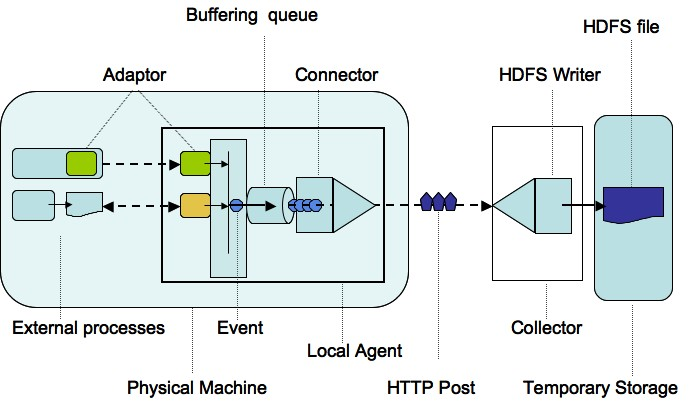
\includegraphics[width=75mm]{chukwa1.jpg}
\caption{The agent side}
\end{figure}
\fi


At the heart of any data collection system is a pipeline to pump data from where it is generated to where it is stored. The requirements at the endpoints dictate the design of the system in the middle. To meet its goals, Chukwa needs flexible, dynamically controllable data sources, and a high performance, large scale storage system. %Generated data ought to be available for processing shortly after generation
 It also needs a suitable framework for analyzing the large volumes of collected data.

\subsection{Adaptors}

Data sources need to be dynamically controllable because the particular data being collected from a machine changes over time, and varies from machine to machine. For example, as Hadoop tasks start and stop, different log files must be monitored. We might want to increase our collection rate if we detect anomalies.  And of course, it makes no sense to collect Hadoop metrics on an NFS server. 

These dynamically controllable data sources are known in Chukwa as \textit{adaptors}, since they generally are wrapping some other data source, such as a file or a Unix command-line tool.  At present, Chukwa includes adaptors to collect Hadoop logs, application metrics, and system telemetry. We expect to write adaptors for tasks like counting recoverable disk read errors, retrieving causal logs from X-Trace \cite{xtrace}, and monitoring operating system and Java virtual machine state.

%\subsection{Adaptors}
% 
%As a result, we bundle data collection into small dynamically loadable Adaptors which run within a local agent process on each machine. This process is left permanently running, and is restarted automatically if it crashes. The agent process is responsible for starting and stopping adaptors in response to external commands.  It also provides two crucial services to adaptors. First, it is responsible for forwarding chunks over HTTP to the collectors, where they are written to stable storage. Second, it is responsible for making regular checkpoints of adaptor state, and restarting adaptors at the appropriate position after a crash.  This checkpoint mechanism ensures that data is appropriately resent after a crash.


\subsection{Storage}

The scalability challenges in large-scale monitoring systems primarily concern the data storage and analysis components, since that is where data from multiple machines is brought together. We determined from the outset to rely on Hadoop's HDFS as our storage component. Hadoop HDFS installations can store petabytes of data, and support high throughput; 20 MB/sec for one writer is typical in operational deployments, with total cluster throughput routinely in excess of a gigabyte per second. HDFS also facilitates parallel processing of stored data with MapReduce.

Unfortunately, HDFS is not designed for the sort of workloads associated with monitoring. HDFS aims to handle large files and high write rates from comparatively small numbers of writers. It is not designed for thousands of concurrent low-rate writers, and millions of small files. Worse, writes to a file are not visible to readers until the file is closed, and stable versions of HDFS do not allow closed files to be reopened for writing. As a result, some care must be taken in using HDFS to support continuous rather than batch processing.
 Much of the Chukwa design was driven by the need to reconcile our many sporadic data sources with HDFS's performance characteristics and semantics.
 
\subsection{Collectors and Agents}

Chukwa resolves these conflicting demands by adding additional pipeline stages between the adaptors and the HDFS data store: \textit{collectors} and \textit{agents}.

Rather than have each adaptor write directly to HDFS, data is sent across the network to a \textit{collector} process, that does the HDFS writes.  Each collector receives data from several hundred hosts, and writes all this data to a single \textit{sink file}, consisting of chunks of data plus metadata describing each chunk's source and format. Periodically, collectors close their sink files, rename them to mark them available for processing, and resume writing a new file.  Data is sent to collectors over HTTP, since this allows us to write our collector as a Java servlet. This in turn lets us use standard Java servlet containers for connection management. This is in keeping with the Chukwa philosophy of leveraging existing infrastructure when possible. 

Collectors thus drastically reduce the number of HDFS files generated by Chukwa, from one per machine or adaptor per unit time, to a handful per cluster.  The decision to put collectors between data sources and the data store has other benefits. Collectors hide the details of the HDFS file system in use, such as its Hadoop version, from the adaptors.  This is a significant aid to configuration.  It is especially helpful when using Chukwa to monitor a development cluster running a different version of Hadoop or when using Chukwa to monitor a non-Hadoop cluster.  

The second of our intermediate stages, agents, are less fundamental to the design. They exist primarily to provide various services to adaptors, and thus to make adaptors easier to write. Agents are long-running processes on each machine being monitored by Chukwa.  Each agent process is restarted automatically if it crashes. The agent provides three chief services to adaptors. First, the agent is responsible for starting and stopping adaptors in response to external commands.
Second, it is responsible for forwarding chunks over HTTP to the collectors, where they are written to stable storage. 
Third, it is responsible for making regular checkpoints of adaptor state, and restarting adaptors at the appropriate position after a crash.  



%FIXME: ruby/failmon

%The output of an adaptor consists of chunks, each containing one or more semantically meaningful records.  These records, such as lines from a log file or batches of metrics, must be kept together.  This means that adaptors must parse files intensively enough to detect record boundaries, and they must correctly handle buffering.

%These costs are offset by important advantages. Keeping records intact allows collectors to run filters or triggers against data streams, without having to buffer partial lines. In the presence of load balancing across collectors, these filters will still behave properly. Perhaps most importantly, this allows the map phase of the periodic MapReduce process to extract metadata from records and use this metadata as a sort key: a large performance win.  If records were split across collectors, this metadata could be inaccessible.

%FIXME: say something here
%After a crash, the local agent restarts each adaptor, passing sequence number of the last byte of their output that was successfully sent to a collector.  Adaptors that read from files can seek to that offset before starting.  Adaptors that output ephemeral data, such as CPU load, can simply begin numbering output from this point, to mask  any crash-induced discontinuity from downstream users. 

%\subsection{Agent}

%Adaptors run within a local agent process on each machine. This checkpoint mechanism ensures that data is appropriately resent after a crash.

%We opted to put most of the recovery logic in the agents, rather than the collectors. This removes state from the collectors. We considered having agents check with collectors to find out what the last thing they sent was. However, each agent would have to check with each collector, resulting in an exorbitant number of connections if many agents fail and reboot simultaneously.


\subsection{Demux and archiving}

A pair of MapReduce jobs runs every few minutes, taking all the available sink files as input.  The first job simply archives all the collected data, without processing or interpreting it.  The second job parses out structured data from some of the logs, and loads this structured data into a data store.  

% For performance reasons, we do record parsing in the Map phase, and extract key-value pairs. Example records include job history reports, task durations, and so forth. We then use the shuffle and sort phases of the Reduce to organize records semantically by application timestamp and type. This forced us to design our adaptors to have adaptors output meaningful records, and not arbitrary chunks of streams. %% FIXME: recast last sentence

 These datastores are also pluggable. For now, we use HDFS files, one file per cluster, per data type, and time period.  So for instance there would be one file for all of a particular clusters datanode logs, for the period from noon to 1pm on a given day.   This is only an interim solution, and we are evaluating various more suitable data stores, with support for structured queries.  Hive, an HDFS-backed data warehouse might also be a good fit here. \cite{hive} 
 % Hive supports a subset of SQL for queries, which is particularly appealing for the context of ad-hoc analytics. 
 Column-oriented databases such as HBase, and Hypertable would also be sensible options.  For small deployments, a local relational database would be suitable.

%This de-multiplexing is the phase of Chukwa processing with the highest latency. Hadoop TaskTrackers only poll for work every few seconds, and therefore map-reduce jobs have an inherent latency larger than that.  Unfortunately, we do need this de-multiplexing stage, since HDFS, and structured stores built on top of it, perform much better for large writes than for small ones.

Data stored in HDFS in a structured format can be processed straightforwardly with MapReduce jobs. We envision a library of ``canned'' MapReduce jobs for tasks like finding common failure modes, correlating events in the logs with slowdowns, discovering flakey machines, and so forth.  Since Chukwa data is split into different files based on content, these jobs take as input only a small fraction of the total data volume, and therefore can run relatively quickly.  Most structured storage systems, including Hive and Hypertable, include their own query interfaces. We expect that these interfaces will be used by users who want to do simple ad-hoc queries over stored Chukwa data, with MapReduce being reserved for more complex processing.

\section{Data Analysis and Display}

Collected data is only as useful as the analysis that can be done on it.  To ease analysis of collected data, we've built a flexible, configurable, ``portal-style'' web interface to Chukwa, termed the Hadoop Infrastructure Care Center (HICC). A configurable interface is not simply a frill --- it is necessary, since different users have very different data analysis needs.

\begin{figure}
% 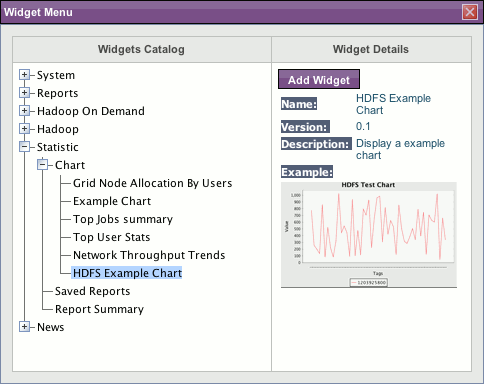
\includegraphics[width=75mm]{widget.png}
%\caption{The HICC widget catalog} 
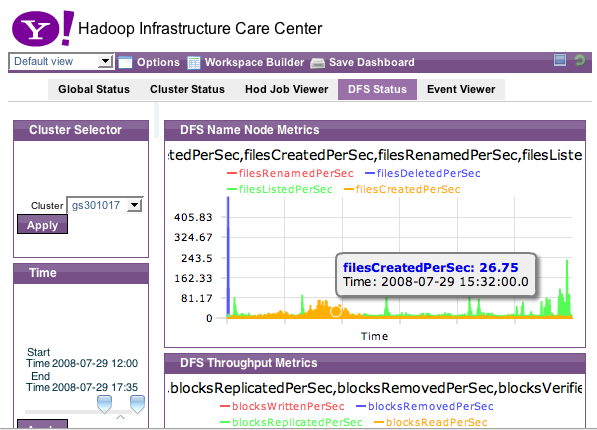
\includegraphics[width=75mm]{hicc_in_action2.png}
\caption{HICC displaying some DataNode metrics}
\end{figure}


In practice, a single individual often fulfills more than one of these roles, or some portion of a role. As a result, there is a compelling need to allow individuals to mix and match different components. We chose to do this by bundling each query, or family of queries, into a widget. HICC users can assemble their HICC workspace by selecting widgets from a catalog, in exactly the way that they can customize their personal Yahoo! or Google portal pages.

Some of these components will display the results of canned map-reduce jobs run against data in  Chukwa storage.  Others will perform on-the-fly queries against SQL databases.    Still others might display telemetry collected with Ganglia, or report on recently opened failure tickets.  

% HICC stores several kinds of widget state.  There is a global context, through which different widgets can ``collaborate'' and share data. There is a dashboard view, which stores information about the user's preferred layout, and display settings.  There is a widget descriptor file, for storing widget configuration and parameters.   

%HICC is not intended for exploratory, ad-hoc queries. For that, we expect to rely on the query interface of our structured data store.  Since this store is not yet available, we have been using a MySQL database.


\section{Evaluation}

%Chukwa is currently in development, and we have not yet been able to do large-scale tests.  However, we have reason to be confident that Chukwa will comfortably meet our performance goals.

Using logs from a production cluster at Yahoo!, we found that a 2000-node production cluster would generate around 5.5 MB of data per second.  Of this, the vast bulk (more than 95\%) was task tracker logs.  Metrics data accounted for more than half the remainder, with Namenode, HDFS datanode, and JobTracker logs accounting for the rest. This data rate is small enough that Chukwa should impose only very modest overhead on datacenter networks. 

We conducted a number of small experiments to verify that Chukwa could handle this load.   All tests were run on an internal development cluster at Yahoo.  Machines had four 2.8 GHz Xeon processors, four IDE disks, and 3 GB of RAM, and ran Linux, with a 2.6.9 kernel.  %kernel version 2.6.9-55
There are two potential bottlenecks in Chukwa that we evaluated in detail, the collector, and the map-reduce job.  At present, collector throughput is more than adequate, and the demux job is the limiting phase in processing.

To measure collector performance, we ran Chukwa on a 400 node test cluster. We configured nodes in this cluster to report data at many times the normal operational rate, emulating a much larger cluster.  In this configuration, the test cluster generated 14.4 megabytes of monitoring data per second.  A single collector was able to keep up with this data volume, and write it to HDFS; in a 30 minute test run, machine utilization never rose much above 50\%.  At this rate, we are bumping into the single-writer throughput limits imposed by HDFS, rather than any Chukwa-specific limits. Higher Chukwa bandwidth could be achieved by simply adding more writers.

%The scalability limits we observed in more intensive experiments were caused by thread limits in Jetty, the Servlet container we are using at present. These limits can likely be overcome by more careful configuration. However, 7.2 MB/sec significantly exceeds both our performance goals and the rate at which we can process incoming data, so we have yet to perform this optimization. 

At present, the rate-limiting phase of Chukwa is the Demux job. Using five worker nodes, our MapReduce job can process two gigabytes of metrics data in around three and a half minutes. We conducted five trials on the same 2 GB of test data.  Completion times ranged from 3:25 minutes to 3:34, with a mean of 3:30.  This means that we can can process six minutes' of incoming data in three and a half minutes, thus keeping up with the incoming data flow and achieving our ten minute target latency.  
Optimizing MapReduce jobs is fairly routine engineering at this point, and we believe that significant gains can be achieved here. 

These results show that Chukwa can maintain latencies well under our ten minute target, while imposing very modest overheads on the cluster: five Chukwa nodes are only 0.25\% of our notional 2000-node cluster. We expect to be able to maintain these latency targets as we scale up the number of nodes being monitored.  Ramping up the size of MapReduce jobs is routine, and the engineering issues are well understood. Even for monitoring hundreds of thousands of nodes, Chukwa's data volumes would be significantly smaller than those seen in our production web indexing clusters.


\section{Related Work}
%\label{sec:related}

Chukwa represents a design point in between two existing classes of systems: log collection frameworks on the one hand, and network management systems on the other.  Chukwa intends to combine the abundance of data display tools of existing NMS systems, with the high throughput and robustness expected of log collection frameworks.

The syslog protocol supported streaming logs across the network as long ago as the late 1980s.  However, syslog had serious defects: no clear solution to the discovery, load balancing, or failure handing problems.  Facebook's Scribe \cite{scribe} system apparently solves some of these problems, but unfortunately, no details of Scribe have been published.

Chukwa has some similarity with network monitoring systems such as Nagios, Ganglia, or Tivoli Monitoring \cite{Ganglia, Nagios, tivmon}. The three systems differ in emphasis, but have important commonalities.  All are capable of collecting and storing substantial volumes of metrics data. All include tools for displaying this data.  Nagios and Tivoli monitoring have centralized architectures, while Ganglia is decentralized.  Ganglia, unfortunately, is heavily adapted towards numeric time-series data, and provides minimal support for the sort of complex text-processing necessary for our applications.

Chukwa, however, differs in crucial respects from these current systems. Today's monitoring systems are focused primarily on collection, with storage being a secondary priority.  Chukwa is designed for far higher data rates; metrics data, which is essentially all that Ganglia and Nagios are used to collect, is only a few percent of the data we will capture in operational settings. 

With hundreds of gigabytes of data being collected per day, processing the stored data becomes a key bottleneck.  Chukwa's design was optimized precisely for storage and batch processing of collected data.  While MapReduce is routinely used at these scales, no currently available monitoring system makes provision for large-scale data intensive processing. 


\section{Conclusion}
%\label{sec:conclusion}

Chukwa demonstrates that a high performance distributed monitoring system can readily be built atop existing distributed data collection frameworks. The Hadoop distributed file system supports petabytes of stored data and hundreds of megabytes per second of write throughput, enough for even very demanding monitoring applications. MapReduce provides a suitable framework for organizing and analyzing these data volumes.

% Chukwa provides flexible and powerful tools for analyzing and displaying collected monitoring data.  We expect Chukwa to be very useful in monitoring and managing large system deployments.

Building Chukwa on top of Hadoop resulted in a few design quirks, and a modest latency penalty.  However, it greatly simplified implementation, and leverages the substantial amount of work going into Hadoop.  Hadoop 0.19, which will be released within a few months, should significantly improve the performance of short-running Map tasks, which will allow us to efficiently operate Chukwa on short timescales.

%\iffalse
%\subsection{Future Work}
%\fi

%\section{Acknowledgments}

\addcontentsline{toc}{section}{References}
\begin{thebibliography}{99}

\bibitem{mapreduce}
Jeffrey Dean and Sanjay Ghemawat. ``MapReduce: Simplified Data Processing on Large Clusters.'' \newblock In \textit{Communications of the ACM}, Volume 51, Issue 1, pp. 107-113, 2008.
\bibitem{Ganglia}
Matthew L. Massie, Brent N. Chun, and David E. Culler.  ``The Ganglia Distributed Monitoring System: Design, Implementation, and Experience''.
\newblock In \textit{Parallel Computing} Volume 30, Issue 7, pp 817-840, 2004.
\bibitem{Nagios}
http://www.nagios.org/
\bibitem{tivmon}
IBM Tivoli Monitoring.
\newblock Available online: \texttt{http://www.ibm.com/ software/ tivoli/ products/ monitor/}
\bibitem{hive}
Joydeep Sen Sarma.  ``Hive as a contrib project''
\newblock Available online: https://issues.apache.org/jira/browse/HADOOP-3601
\bibitem{xtrace}
Rodrigo Fonseca, George Porter, Randy H. Katz, Scott Shenker, and Ion Stoica.  X-Trace: A Pervasive Network Tracing Framework.
\newblock In \textit{4th USENIX Symposium on Networked Systems Design \& Implementation (NSDI'07)}, Cambridge, MA, USA, April 2007.
\bibitem{scribe}
Scribe logfile aggregation system described by Facebook's Jeff Hammerbacher
\url{https://issues.apache.org/jira/browse/HADOOP-2206?focusedCommentId=12542775#action_12542775}

\end{thebibliography}

\end{document}

%		TODO:
%	Maybe more depth in related work
%	More performance numbers
%	Mention "work in progress" somewhere up front?
%	Better screen shot for HICC



